%%%%%%%%%%%%%%%%%%%%%%%
%% Folie             %%
%%%%%%%%%%%%%%%%%%%%%%%
\begin{frame}
    \frametitle{Deep Reinforcement Learning}

\begin{PraesentationAufzaehlung}
    \item Learns to solve tasks by maximize the reward signal it gets
    \item But there are some task that seems to be very hard to learn from scratch, where one wrong decision has catastrophic results in the end
\end{PraesentationAufzaehlung}

\end{frame}
\clearpage


%%%%%%%%%%%%%%%%%%%%%%%
%% Folie             %%
%%%%%%%%%%%%%%%%%%%%%%%
\begin{frame}
    \frametitle{What we want}

\begin{multicols}{2}
	An Agent who know how to
	\begin{PraesentationAufzaehlung}
		\item Prevent dangerous situations
		\item Get bonus points
		\item Get them as fast as possible
	\end{PraesentationAufzaehlung}
	We want an agent who is acting with foresight
    \vfill\columnbreak
	\begin{center}
    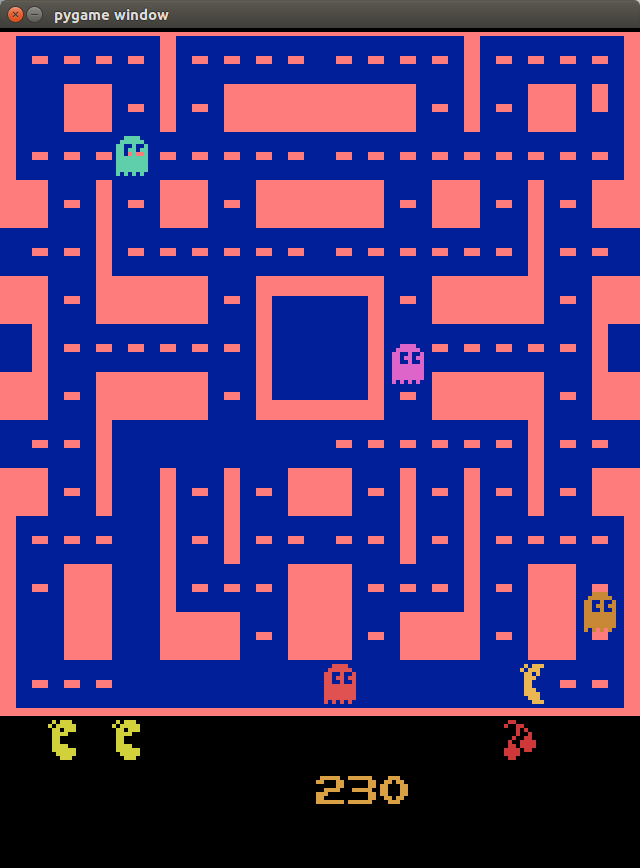
\includegraphics[height=.6\textheight]{./Images/screenshot_ghost.png}%
	\end{center}
\end{multicols}


\end{frame}
\clearpage



%%%%%%%%%%%%%%%%%%%%%%%
%% Folie             %%
%%%%%%%%%%%%%%%%%%%%%%%
%\begin{frame}
%    \frametitle{Goals}

%\begin{PraesentationAufzaehlung}
%    \item Working Implementation of I2A in pytorch
%\end{PraesentationAufzaehlung}

%\end{frame}
%\clearpage

%%%%%%%%%%%%%%%%%%%%%%%%%%%%%%%%%%%%%%%%%%%%%%%%%%%%%  
 % FOLIENSTIL: Weisse Schrift auf blauem Grund 
\PraesentationMasterWeissBlau 
\begin{frame} 
    \PraesentationUeberschriftZweizeilig{Imagination-Augmented Agent (I2A)}{Weber et al. (2017)}

\end{frame} 

\PraesentationMasterStandard


%%%%%%%%%%%%%%%%%%%%%%%
%% Folie             %%
%%%%%%%%%%%%%%%%%%%%%%%
\begin{frame}
    \frametitle{Imagination-Augmented Agent (I2A)}

\begin{PraesentationAufzaehlung}
	\item Weber et al.(2017)
    \item Imaginate the future and learn to do better action based on the imaginatied future
    \item Combine model-free and model-based aspects
    \item Architecture for deep reinforcement learning
\end{PraesentationAufzaehlung}

\end{frame}
\clearpage

%%%%%%%%%%%%%%%%%%%%%%%%%%%%%%%%%%%%%%%%
%% Folie: Bilder                      %%
%%%%%%%%%%%%%%%%%%%%%%%%%%%%%%%%%%%%%%%%
\begin{frame}
    \frametitle{I2A Architecture}


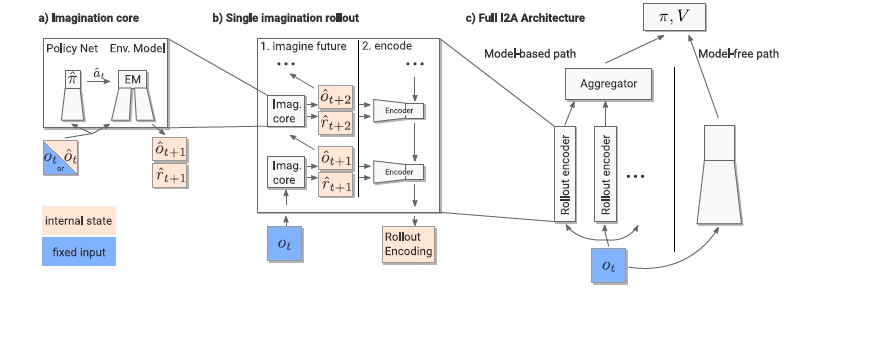
\includegraphics[width=\columnwidth]{./Images/i2a_architecture.png}%
\begin{PraesentationAufzaehlung}
	\item Input observation $o_t$
	\item Output policy $\pi$ and value function $V$
\end{PraesentationAufzaehlung}
    
\end{frame}
\clearpage

%%%%%%%%%%%%%%%%%%%%%%%%%%%%%%%%%%%%%%%%
%% Folie: Bilder - Zweispaltige Seite %%
%%%%%%%%%%%%%%%%%%%%%%%%%%%%%%%%%%%%%%%%
\begin{frame}
    \frametitle{Training I2A}

\begin{multicols}{2}
	\begin{PraesentationAufzaehlung}
	    \item Learn policy $\pi$ and value function $V$
		\item Train with Advantage-Actor-Critic (A2C)
	\end{PraesentationAufzaehlung}
    \vfill\columnbreak
	\begin{center}
    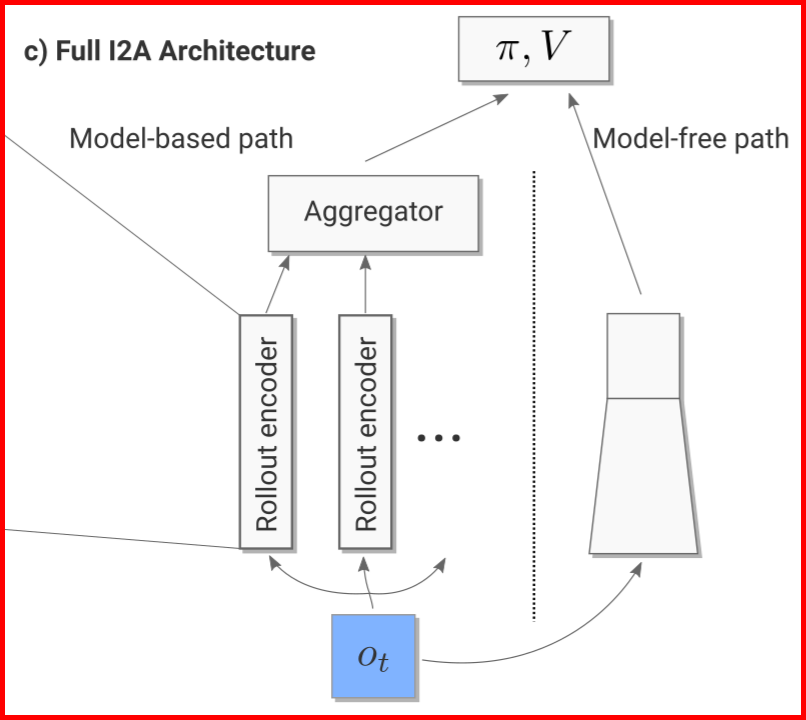
\includegraphics[width=\columnwidth]{./Images/i2a_a2c.png}%
	\end{center}
\end{multicols}
    
\end{frame}
\clearpage

%%%%%%%%%%%%%%%%%%%%%%%
%% Folie             %%
%%%%%%%%%%%%%%%%%%%%%%%
\begin{frame}
    \frametitle{Advantage-Actor-Critic (A2C)}

\begin{PraesentationAufzaehlung}
    \item Actor	learns policy function $\mathnormal{\pi(s, a, \theta)}$:\\
	Controls how the agent acts\\
	Policy update:
	\begin{equation}
	\mathnormal{\nabla \theta = \alpha \nabla_\theta (log \pi_\theta (s, a)) q_w (s, a)}
	\end{equation}	
	\item Critic learns value function $\mathnormal{V(s, a, w)}$:\\
	Messures how good a choosen actions is\\
	Value update:
	\begin{equation}
	\mathnormal{
	\nabla w = \beta (R(s, a) + \gamma q_w(s_{t+1}, a_{t+1}) - q_w(s_t, a_t)) \nabla_w q_w(s_t, a_t)}
	\end{equation}
\end{PraesentationAufzaehlung}

\end{frame}
\clearpage


%%%%%%%%%%%%%%%%%%%%%%%%%%%%%%%%%%%%%%%%
%% Folie: Bilder                      %%
%%%%%%%%%%%%%%%%%%%%%%%%%%%%%%%%%%%%%%%%
\begin{frame}
    \frametitle{I2A Architecture - Model Free Path}


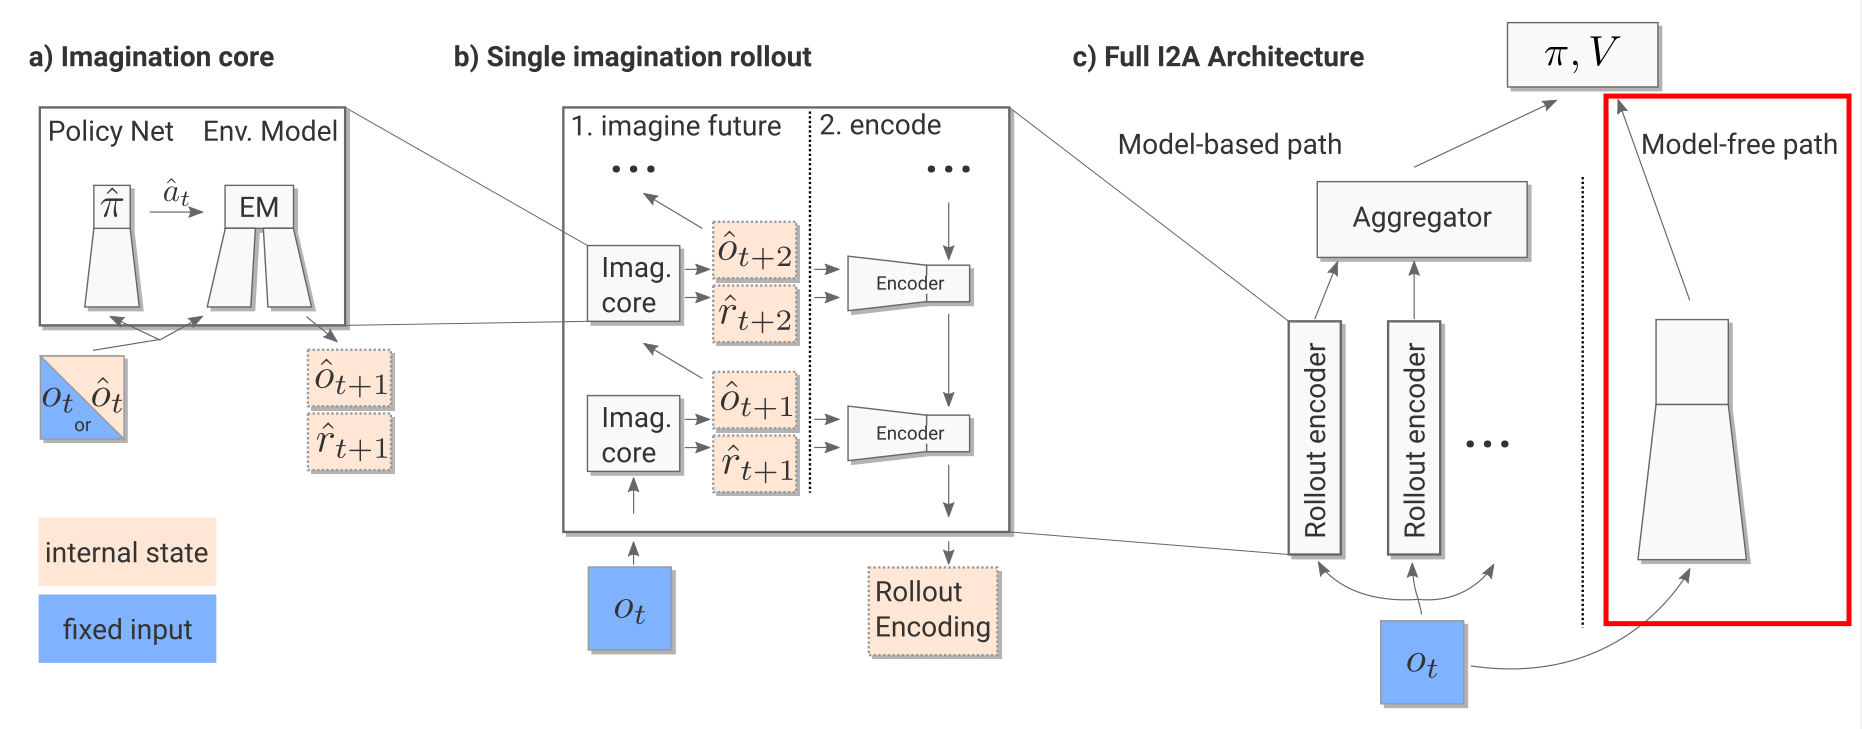
\includegraphics[width=\columnwidth]{./Images/i2a_all_model_free_path.png}%

\begin{PraesentationAufzaehlung}
	\item CNN Layers followed by Fully Connected Layers as usually used for Reinforcement Learning
\end{PraesentationAufzaehlung}

\end{frame}
\clearpage

%%%%%%%%%%%%%%%%%%%%%%%%%%%%%%%%%%%%%%%%
%% Folie: Bilder - Zweispaltige Seite %%
%%%%%%%%%%%%%%%%%%%%%%%%%%%%%%%%%%%%%%%%
%\begin{frame}
%    \frametitle{I2A Architecture - Model Free Path}

%\begin{multicols}{2}
%	\begin{PraesentationAufzaehlung}
%		\item 
%	\end{PraesentationAufzaehlung}
%    \vfill\columnbreak
%	\begin{center}
%    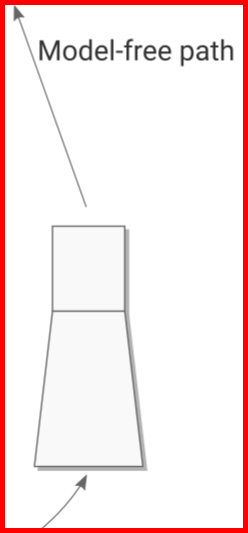
\includegraphics[height=.5\textheight]{./Images/i2a_model_free_path.png}%
%	\end{center}
%\end{multicols}
%    
%\end{frame}
%\clearpage


%%%%%%%%%%%%%%%%%%%%%%%%%%%%%%%%%%%%%%%%
%% Folie: Bilder                      %%
%%%%%%%%%%%%%%%%%%%%%%%%%%%%%%%%%%%%%%%%
\begin{frame}
    \frametitle{I2A Architecture - Model Based Path}


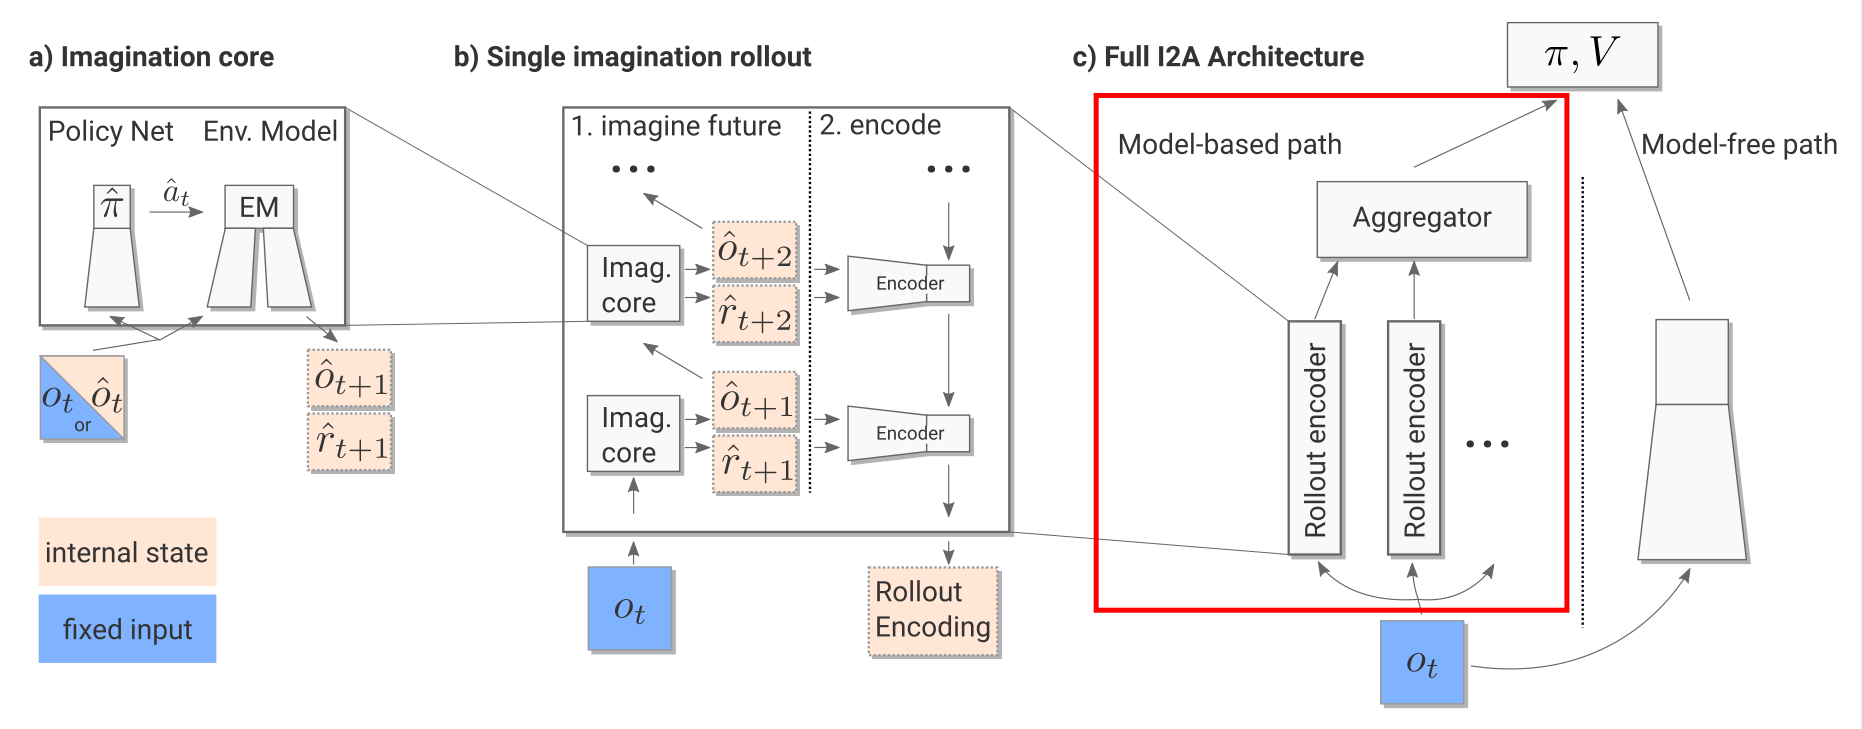
\includegraphics[width=\columnwidth]{./Images/i2a_all_model_based_path.png}%

\begin{PraesentationAufzaehlung}
	\item Imaginate the Future based on an model of the environment and use this information for decision making
\end{PraesentationAufzaehlung}
    
\end{frame}
\clearpage

%%%%%%%%%%%%%%%%%%%%%%%%%%%%%%%%%%%%%%%%
%% Folie: Bilder - Zweispaltige Seite %%
%%%%%%%%%%%%%%%%%%%%%%%%%%%%%%%%%%%%%%%%
\begin{frame}
    \frametitle{I2A Architecture - Model Based Path}

\begin{multicols}{2}
	\begin{PraesentationAufzaehlung}
	    \item Rollout encoder:\\
		For each action the agent can take 
		imaginate the future% and learn relevent information that can happen
		\item Aggregator: \\
		Concatinate all action rollouts
	\end{PraesentationAufzaehlung}
    \vfill\columnbreak
	\begin{center}
    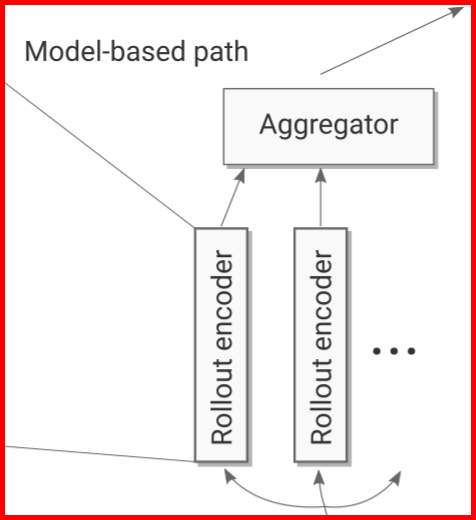
\includegraphics[height=.5\textheight]{./Images/i2a_model_based.png}%
	\end{center}
\end{multicols}
    
\end{frame}
\clearpage



%%%%%%%%%%%%%%%%%%%%%%%%%%%%%%%%%%%%%%%%
%% Folie: Bilder                      %%
%%%%%%%%%%%%%%%%%%%%%%%%%%%%%%%%%%%%%%%%
\begin{frame}
    \frametitle{I2A Architecture - Imagination Rollout}


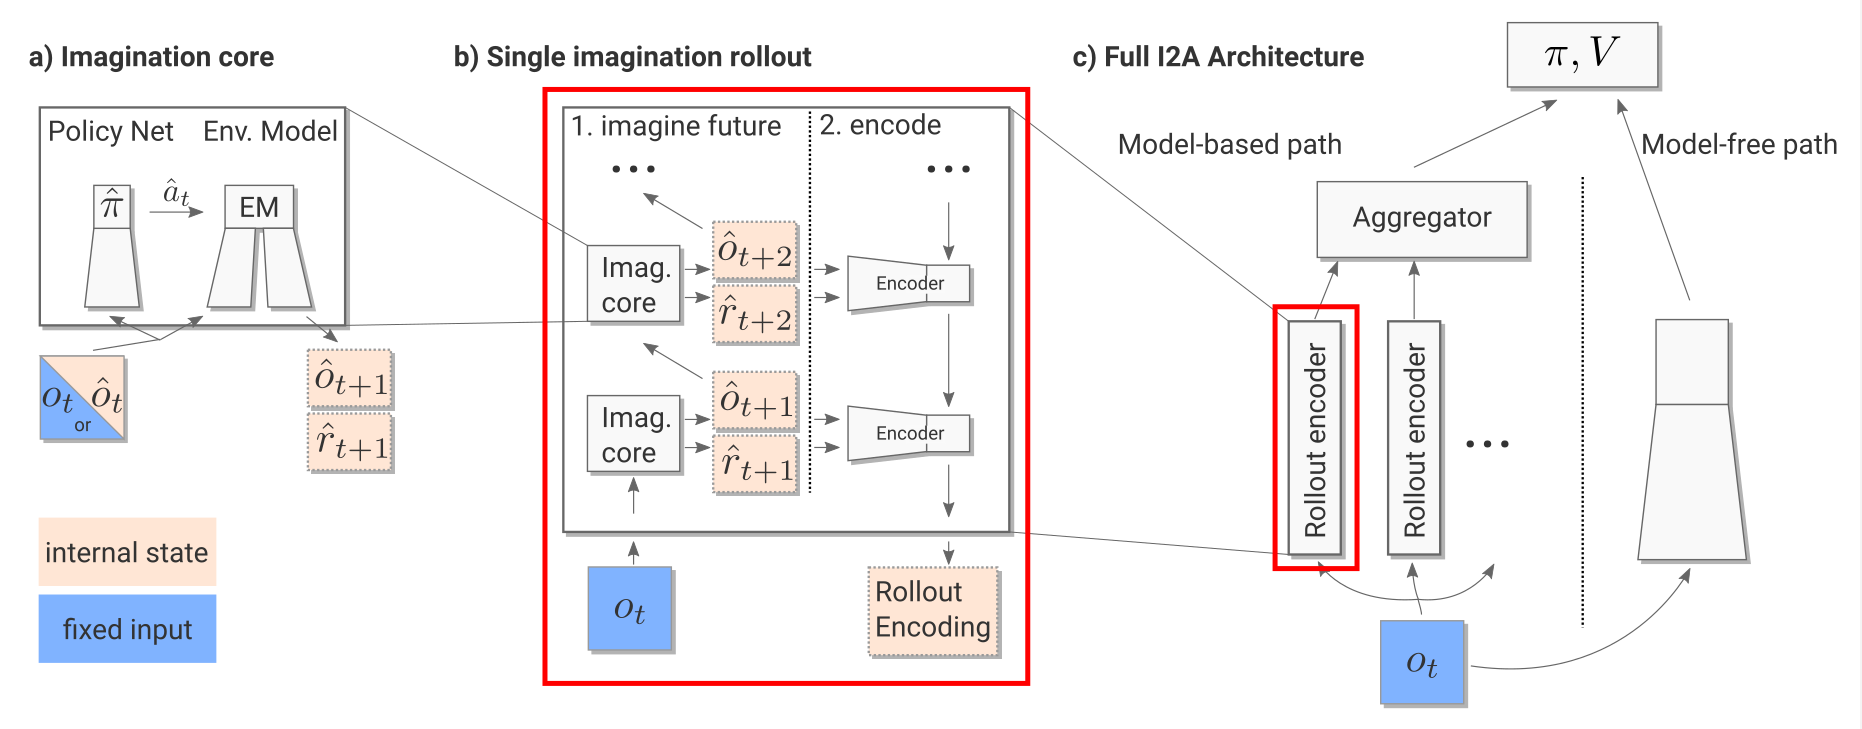
\includegraphics[width=\columnwidth]{./Images/i2a_all_imagination_rollout.png}%

\begin{PraesentationAufzaehlung}
	\item Predict what will happen in the future
\end{PraesentationAufzaehlung}
    
\end{frame}
\clearpage


%%%%%%%%%%%%%%%%%%%%%%%%%%%%%%%%%%%%%%%%
%% Folie: Bilder - Zweispaltige Seite %%
%%%%%%%%%%%%%%%%%%%%%%%%%%%%%%%%%%%%%%%%
\begin{frame}
    \frametitle{I2A Architecture - Imagination Future}

\begin{multicols}{2}
	\begin{PraesentationAufzaehlung}
		\item Input:\\
		observation $o_t$ and start action $a$
		\item Output:\\
		n imagined trajectories ($o_{t+i}, r_{t+i}$ for $i = 0, ..., n$)
	\end{PraesentationAufzaehlung}
    \vfill\columnbreak
	\begin{center}
    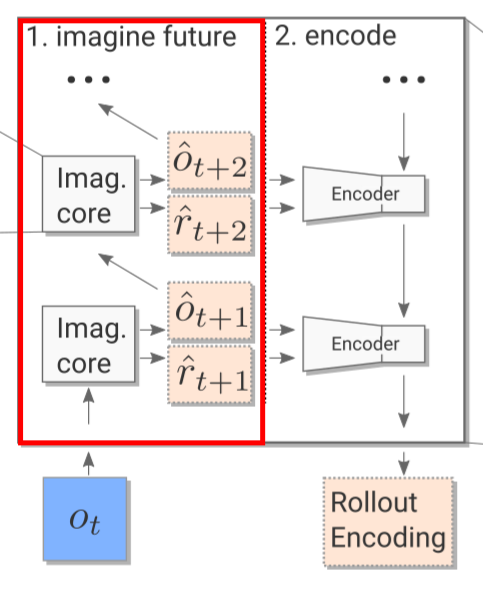
\includegraphics[height=.5\textheight]{./Images/imagine_future.png}%
	\end{center}
\end{multicols}
    
\end{frame}
\clearpage

%%%%%%%%%%%%%%%%%%%%%%%%%%%%%%%%%%%%%%%%
%% Folie: Bilder - Zweispaltige Seite %%
%%%%%%%%%%%%%%%%%%%%%%%%%%%%%%%%%%%%%%%%
\begin{frame}
    \frametitle{I2A Architecture - Encoder}

\begin{multicols}{2}
	\begin{PraesentationAufzaehlung}
		\item CNN Network followed by an LSTM Network
		\item Learns usefull information from the rollout trajectories
	\end{PraesentationAufzaehlung}
    \vfill\columnbreak
	\begin{center}
    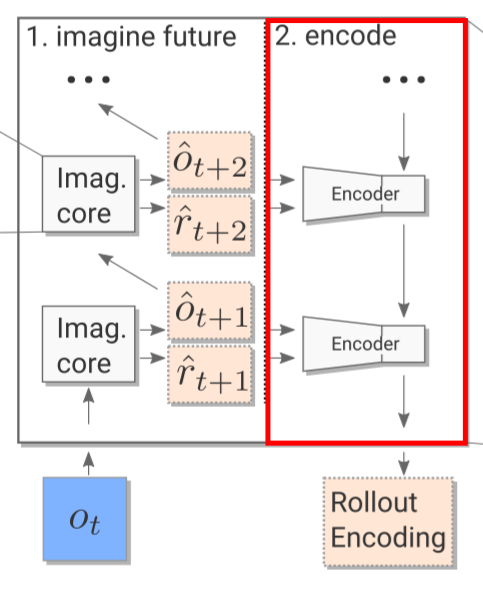
\includegraphics[height=.5\textheight]{./Images/encoder.png}%
	\end{center}
\end{multicols}
    
\end{frame}
\clearpage

%%%%%%%%%%%%%%%%%%%%%%%%%%%%%%%%%%%%%%%%
%% Folie: Bilder                      %%
%%%%%%%%%%%%%%%%%%%%%%%%%%%%%%%%%%%%%%%%
\begin{frame}
    \frametitle{I2A Architecture - Imagination Core}


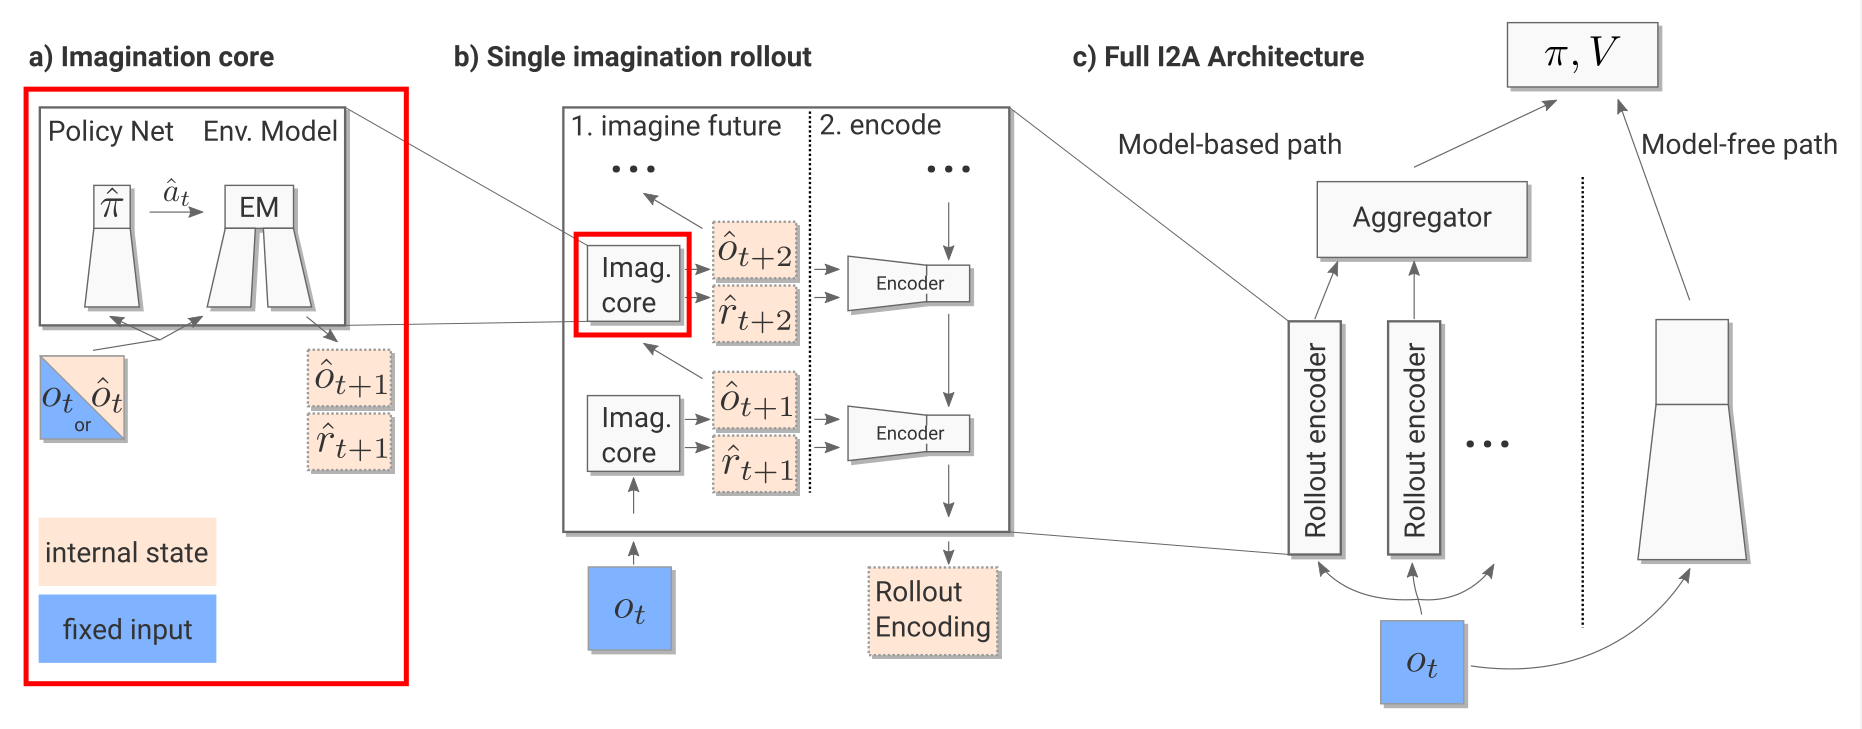
\includegraphics[width=\columnwidth]{./Images/i2a_all_imagination_core.png}%

Imaginate the next observation $o_{t+i}$ and next reward $r_{t+i}$ given observation $o_t$
\end{frame}
\clearpage


%%%%%%%%%%%%%%%%%%%%%%%%%%%%%%%%%%%%%%%%
%% Folie: Bilder - Zweispaltige Seite %%
%%%%%%%%%%%%%%%%%%%%%%%%%%%%%%%%%%%%%%%%
%\begin{frame}
%    \frametitle{I2A Architecture - Imagination Core}

%\begin{multicols}{2}
%	\begin{PraesentationAufzaehlung}
%		\item Imaginate the next observation $o_{t+i}$ and next reward $r_{t+i}$ given observation $o_t$
%	\end{PraesentationAufzaehlung}
%    \vfill\columnbreak
%	\begin{center}
%    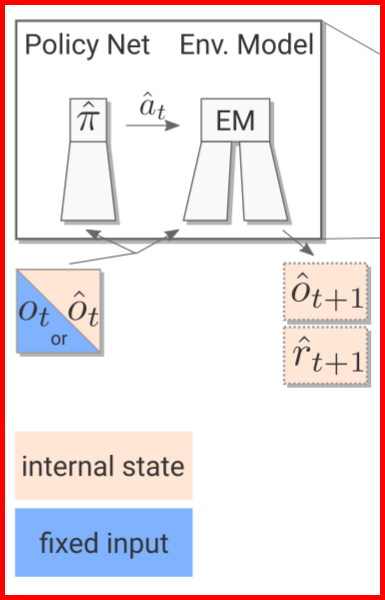
\includegraphics[height=0.5\textheight]{./Images/i2a_imagination_core.png}%
%	\end{center}
%\end{multicols}
    
%\end{frame}
%\clearpage

%%%%%%%%%%%%%%%%%%%%%%%%%%%%%%%%%%%%%%%%
%% Folie: Bilder - Zweispaltige Seite %%
%%%%%%%%%%%%%%%%%%%%%%%%%%%%%%%%%%%%%%%%
\begin{frame}
    \frametitle{I2A Architecture - Imagination Core Policy Network}

\begin{multicols}{2}
	\begin{PraesentationAufzaehlung}
	    \item Policy network $\hat{\pi}$ desides the next action $a_t$
		\item Add distill loss to a2c training to make $\hat{\pi}$ (rollout policy) and $\pi$ (i2a policy) similar
	\end{PraesentationAufzaehlung}
    \vfill\columnbreak
	\begin{center}
    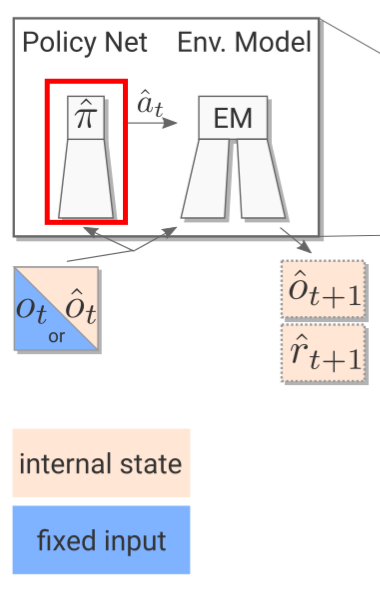
\includegraphics[height=0.5\textheight]{./Images/policy.png}%
	\end{center}
\end{multicols}
    
\end{frame}
\clearpage




%%%%%%%%%%%%%%%%%%%%%%%%%%%%%%%%%%%%%%%%%%%%%%%%%%%%%  
 % FOLIENSTIL: Weisse Schrift auf blauem Grund 
\PraesentationMasterWeissBlau 
\begin{frame} 
    \frametitle{Environment Model}
\end{frame}

\PraesentationMasterStandard

%%%%%%%%%%%%%%%%%%%%%%%%%%%%%%%%%%%%%%%%
%% Folie: Bilder - Zweispaltige Seite %%
%%%%%%%%%%%%%%%%%%%%%%%%%%%%%%%%%%%%%%%%
\begin{frame}
    \frametitle{Environment Model EM}

\begin{multicols}{2}
	\begin{PraesentationAufzaehlung}
		\item Imaginate what will happen if we are in state $o_t$ and do action $a_t$
	\end{PraesentationAufzaehlung}
    \vfill\columnbreak
	\begin{center}
    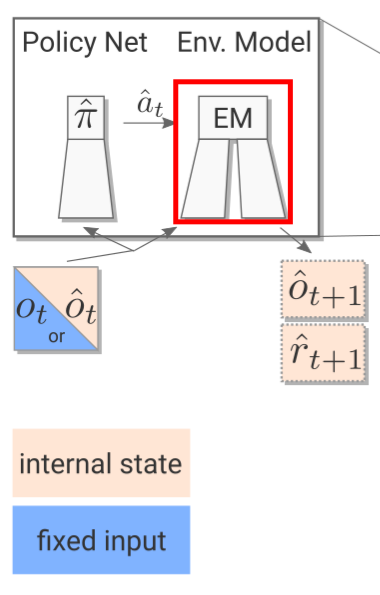
\includegraphics[height=0.5\textheight]{./Images/environment_model.png}%
	\end{center}
\end{multicols}
    
\end{frame}
\clearpage


%%%%%%%%%%%%%%%%%%%%%%%%%%%%%%%%%%%%%%%%
%% Folie: Bilder - Zweispaltige Seite %%
%%%%%%%%%%%%%%%%%%%%%%%%%%%%%%%%%%%%%%%%
\begin{frame}
    \frametitle{Environment Model Architecture}

\begin{multicols}{2}
	\begin{PraesentationAufzaehlung}
		\item kind of Autoencoder
		\item input:\\
		stack of last 3 observations\\
		action as one hot vector\\
		trained with rollouts from a pretrained a2c policy
	\end{PraesentationAufzaehlung}
    \vfill\columnbreak
	\begin{center}
    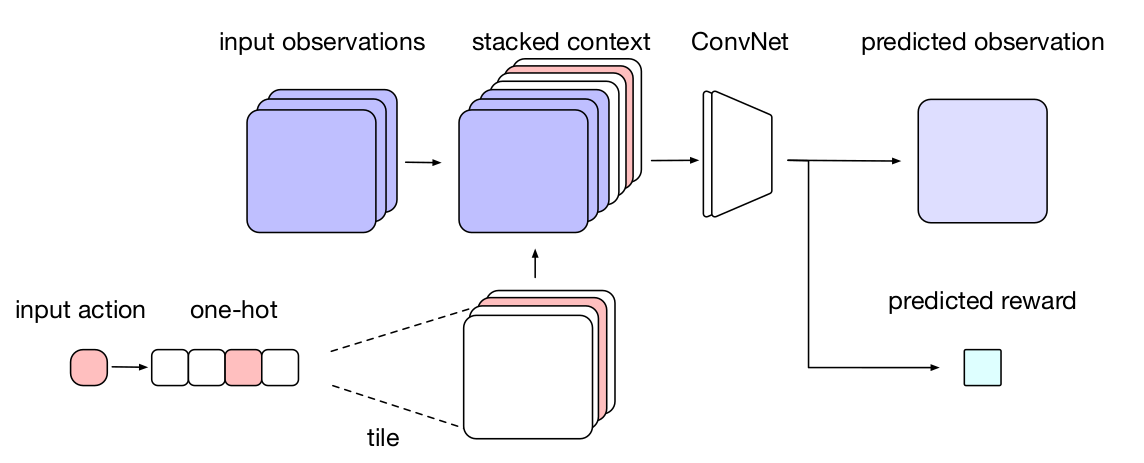
\includegraphics[width=\columnwidth]{./Images/environment_model_architecture.png}%
	\end{center}
\end{multicols}
    
\end{frame}
\clearpage




%%%%%%%%%%%%%%%%%%%%%%%%%%%%%%%%%%%%%%%%
%% Folie: Bilder - Zweispaltige Seite %%
%%%%%%%%%%%%%%%%%%%%%%%%%%%%%%%%%%%%%%%%
\begin{frame}
    \frametitle{Training Environment Model}

\begin{PraesentationAufzaehlung}
	\item Loss:\\
	\begin{equation}
	\mathnormal{
	log p(x, y) }
	\end{equation}
\end{PraesentationAufzaehlung}
    
\end{frame}
\clearpage


%%%%%%%%%%%%%%%%%%%%%%%%%%%%%%%%%%%%%%%%%%%%%%%%%%%%%  
 % FOLIENSTIL: Weisse Schrift auf blauem Grund 
\PraesentationMasterWeissBlau 
\begin{frame} 
    \frametitle{MiniPacman}
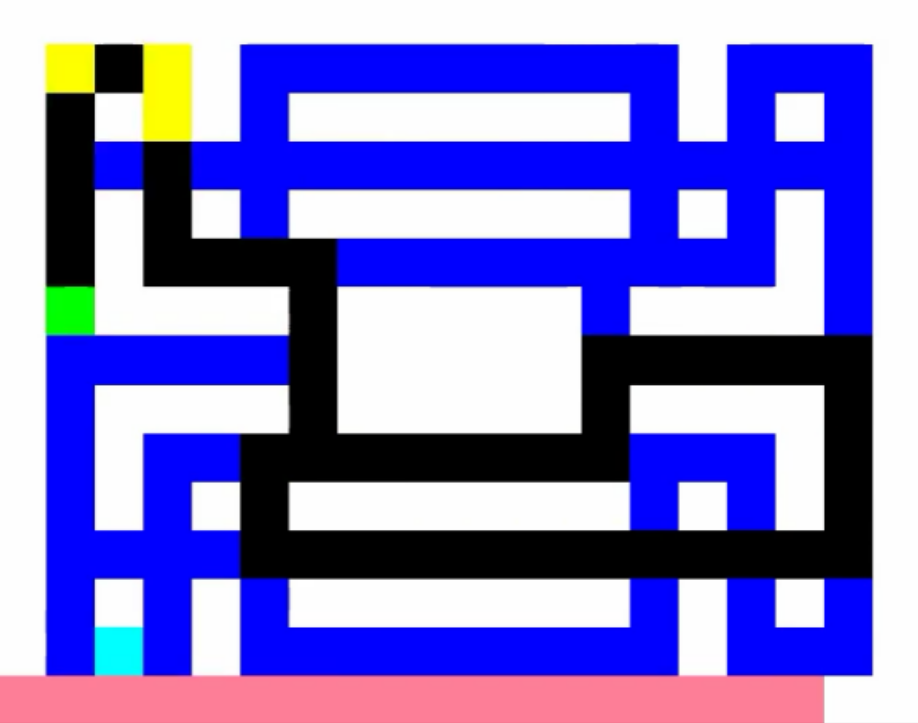
\includegraphics[height=0.5\textheight]{./Images/mini_pacman.png}%
\end{frame} 

\PraesentationMasterStandard

%%%%%%%%%%%%%%%%%%%%%%%%%%%%%%%%%%%%%%%%
%% Folie: Bilder - Zweispaltige Seite %%
%%%%%%%%%%%%%%%%%%%%%%%%%%%%%%%%%%%%%%%%
\begin{frame}
    \frametitle{MiniPacman}

\begin{PraesentationAufzaehlung}
	\item 15 * 19 Grid World
	\item different modes
\end{PraesentationAufzaehlung}
    
\end{frame}
\clearpage




